%\documentclass[11pt,letterpaper,oneside]{article}
\documentclass{article}
%%%% Conditional for including/excluding answers
\newif\ifanswers
\answerstrue %
\answersfalse % comment out to hide answers

\usepackage{Sweave}
\usepackage{moreverb}
\usepackage{amsmath}
\usepackage{graphicx}
\usepackage{verbatim}
\usepackage{alltt}
\usepackage{moreverb}
\usepackage{enumitem}
\usepackage[latin1]{inputenc}
\newcommand\bcdot{\ensuremath{%
  \mathchoice%
   {\mskip\thinmuskip\lower0.2ex\hbox{\scalebox{1.5}{$\cdot$}}\mskip\thinmuskip}}%
   {\mskip\thinmuskip\lower0.2ex\hbox{\scalebox{1.5}{$\cdot$}}\mskip\thinmuskip}%        
   {\lower0.3ex\hbox{\scalebox{1.2}{$\cdot$}}}%  
   {\lower0.3ex\hbox{\scalebox{1.2}{$\cdot$}}}%
}
\title{Introduction to R\\Initial Analysis of Diabetes Data}
\author{Peter Kempthorne  }
\date{Spring 2018}
\begin{document}
\input{RProject1_IntroToR_Diabetes-concordance}
\maketitle

 Consider the diabetes data used by Efron, Hastie, Johnstone and Tibshirani (2004):\footnote{Least Angle Regression, {\it Annals of Statistics}, 2004, Vol 32, No. 2 407-499}
 observations on 442 patients, with the response of interest being a quantitative measure of disease progression one year after baseline. 
There are ten baseline variables---age, sex, body-mass index, average blood pressure, and six blood serum measurements. 


In this note we use this data to illustrate the following basic R functions:

\vspace*{.5in}

\begin{tabular}{ll}
R Function & Purpose/description\\ \hline
$read.csv()$ & Read in data set from a csv file \\
$dim()$ & Display dimensions of matrix/array/data frame \\
$head()$ and $tail()$ & Display top and bottom rows of data\\
$str()$ & Compact display an object's structure\\
$apply()$ & Apply function fixing array margin/dimension\\
$cbind()$ & Bind together column vectors into matrix\\
$data.frame()$ & Create data frame from matrix objects\\
$mean(), var()$ & Compute sample mean and sample variance\\
$cor()$ & Compute correlation matrix \\
$round(,digits=2)$ & Display values rounding to 2 decimal places\\
$par(mfcol=c(2,3))$ & Create 2x3 panel for plots (column ordered)\\
$plot()$ & Generic X-Y  plot \\
$lm()$ & Fit linear model by least squares \\
$summary()$ & Summary statistics for object (e.g., lm fit)\\
\end{tabular}

\newpage


\begin{Schunk}
\begin{Sinput}
> # 1.  Read data into R ----
> diabetes= read.csv(file="EfronData/diabetes.csv", sep=",", header=TRUE)
> #   Display attributes of data frame
> dim(diabetes)
\end{Sinput}
\begin{Soutput}
[1] 442  11
\end{Soutput}
\begin{Sinput}
> head(diabetes)
\end{Sinput}
\begin{Soutput}
  age sex  bmi map  tc   ldl hdl tch  ltg glu prog
1  59   1 32.1 101 157  93.2  38   4 2.11  87  151
2  48   0 21.6  87 183 103.2  70   3 1.69  69   75
3  72   1 30.5  93 156  93.6  41   4 2.03  85  141
4  24   0 25.3  84 198 131.4  40   5 2.12  89  206
5  50   0 23.0 101 192 125.4  52   4 1.86  80  135
6  23   0 22.6  89 139  64.8  61   2 1.82  68   97
\end{Soutput}
\begin{Sinput}
> tail(diabetes)
\end{Sinput}
\begin{Soutput}
    age sex  bmi   map  tc   ldl hdl  tch  ltg glu prog
437  33   0 19.5  80.0 171  85.4  75 2.00 1.72  80   48
438  60   1 28.2 112.0 185 113.8  42 4.00 2.16  93  178
439  47   1 24.9  75.0 225 166.0  42 5.00 1.93 102  104
440  60   1 24.9  99.7 162 106.6  43 3.77 1.79  95  132
441  36   0 30.0  95.0 201 125.2  42 4.79 2.23  85  220
442  36   0 19.6  71.0 250 133.2  97 3.00 2.00  92   57
\end{Soutput}
\begin{Sinput}
> #   Use str() to display structure
> str(diabetes)
\end{Sinput}
\begin{Soutput}
'data.frame':	442 obs. of  11 variables:
 $ age : int  59 48 72 24 50 23 36 66 60 29 ...
 $ sex : int  1 0 1 0 0 0 1 1 1 0 ...
 $ bmi : num  32.1 21.6 30.5 25.3 23 22.6 22 26.2 32.1 30 ...
 $ map : num  101 87 93 84 101 89 90 114 83 85 ...
 $ tc  : int  157 183 156 198 192 139 160 255 179 180 ...
 $ ldl : num  93.2 103.2 93.6 131.4 125.4 ...
 $ hdl : num  38 70 41 40 52 61 50 56 42 43 ...
 $ tch : num  4 3 4 5 4 2 3 4.55 4 4 ...
 $ ltg : num  2.11 1.69 2.03 2.12 1.86 1.82 1.72 1.85 1.94 2.34 ...
 $ glu : int  87 69 85 89 80 68 82 92 94 88 ...
 $ prog: int  151 75 141 206 135 97 138 63 110 310 ...
\end{Soutput}
\begin{Sinput}
> # 2. Compute summary statistics ----
> apply(diabetes,2,summary)
\end{Sinput}
\begin{Soutput}
            age       sex      bmi       map       tc      ldl      hdl
Min.    19.0000 0.0000000 18.00000  62.00000  97.0000  41.6000 22.00000
1st Qu. 38.2500 0.0000000 23.20000  84.00000 164.2500  96.0500 40.25000
Median  50.0000 0.0000000 25.70000  93.00000 186.0000 113.0000 48.00000
Mean    48.5181 0.4683258 26.37579  94.64661 189.1403 115.4391 49.78846
3rd Qu. 59.0000 1.0000000 29.27500 105.00000 209.7500 134.5000 57.75000
Max.    79.0000 1.0000000 42.20000 133.00000 301.0000 242.4000 99.00000
             tch      ltg       glu     prog
Min.    2.000000 1.410000  58.00000  25.0000
1st Qu. 3.000000 1.860000  83.25000  87.0000
Median  4.000000 2.005000  91.00000 140.5000
Mean    4.070249 2.015747  91.26018 152.1335
3rd Qu. 5.000000 2.170000  98.00000 211.5000
Max.    9.090000 2.650000 124.00000 346.0000
\end{Soutput}
\begin{Sinput}
> cbind(mean=apply(diabetes,2,mean), 
+       sd=sqrt(apply(diabetes,2,var)))
\end{Sinput}
\begin{Soutput}
            mean         sd
age   48.5180995 13.1090278
sex    0.4683258  0.4995612
bmi   26.3757919  4.4181216
map   94.6466063 13.8319998
tc   189.1402715 34.6080517
ldl  115.4391403 30.4130810
hdl   49.7884615 12.9342022
tch    4.0702489  1.2904499
ltg    2.0157466  0.2270465
glu   91.2601810 11.4963347
prog 152.1334842 77.0930045
\end{Soutput}
\begin{Sinput}
> round(cor(diabetes),digits=2)
\end{Sinput}
\begin{Soutput}
       age   sex   bmi   map   tc   ldl   hdl   tch   ltg   glu  prog
age   1.00  0.17  0.19  0.34 0.26  0.22 -0.08  0.20  0.27  0.30  0.19
sex   0.17  1.00  0.09  0.24 0.04  0.14 -0.38  0.33  0.15  0.21  0.04
bmi   0.19  0.09  1.00  0.40 0.25  0.26 -0.37  0.41  0.45  0.39  0.59
map   0.34  0.24  0.40  1.00 0.24  0.19 -0.18  0.26  0.39  0.39  0.44
tc    0.26  0.04  0.25  0.24 1.00  0.90  0.05  0.54  0.52  0.33  0.21
ldl   0.22  0.14  0.26  0.19 0.90  1.00 -0.20  0.66  0.32  0.29  0.17
hdl  -0.08 -0.38 -0.37 -0.18 0.05 -0.20  1.00 -0.74 -0.40 -0.27 -0.39
tch   0.20  0.33  0.41  0.26 0.54  0.66 -0.74  1.00  0.62  0.42  0.43
ltg   0.27  0.15  0.45  0.39 0.52  0.32 -0.40  0.62  1.00  0.46  0.57
glu   0.30  0.21  0.39  0.39 0.33  0.29 -0.27  0.42  0.46  1.00  0.38
prog  0.19  0.04  0.59  0.44 0.21  0.17 -0.39  0.43  0.57  0.38  1.00
\end{Soutput}
\end{Schunk}
\begin{Schunk}
\begin{Sinput}
> par(mfcol=c(3,2))
> names(diabetes)
\end{Sinput}
\begin{Soutput}
 [1] "age"  "sex"  "bmi"  "map"  "tc"   "ldl"  "hdl"  "tch"  "ltg"  "glu" 
[11] "prog"
\end{Soutput}
\begin{Sinput}
> #   Plot prog versus age, bmi
> plot(prog ~ age, data=diabetes)
> plot(prog ~ sex, data=diabetes)
> plot(prog ~ bmi, data=diabetes)
> plot(prog ~ map, data=diabetes)
> plot(prog ~ tc, data=diabetes)
> plot(prog ~ ldl, data=diabetes)
\end{Sinput}
\end{Schunk}
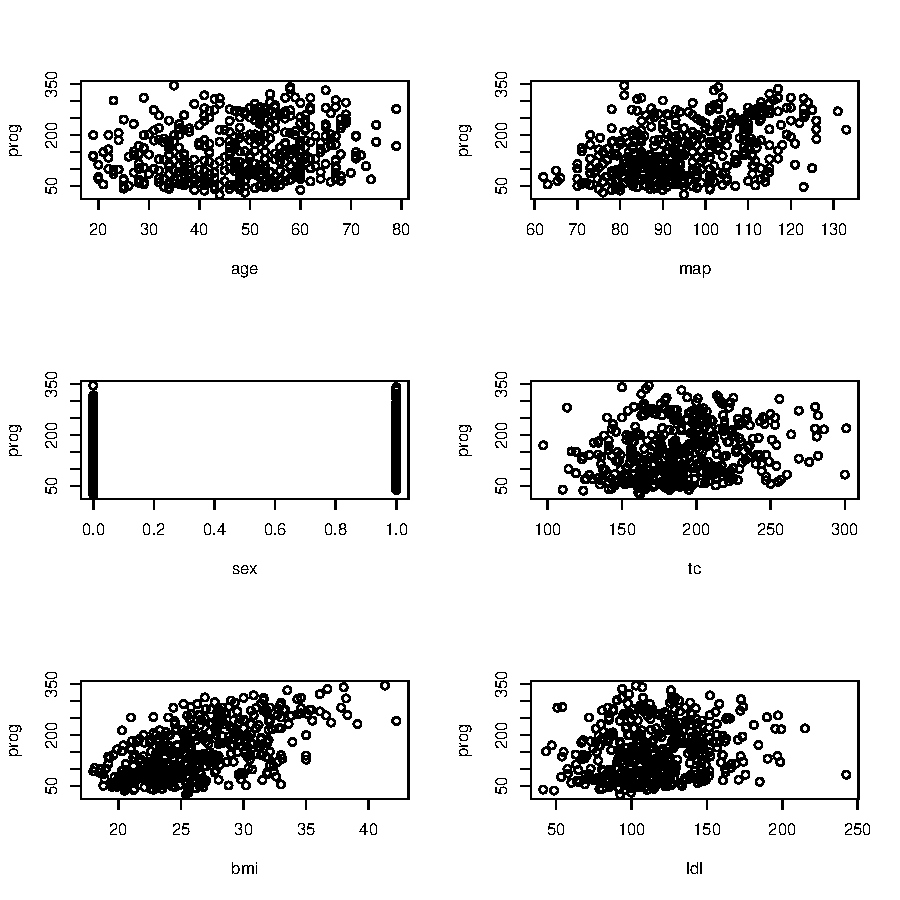
\includegraphics{RProject1_IntroToR_Diabetes-002}
\begin{Schunk}
\begin{Sinput}
> # 3.  Fit linear regression model ----
> lmfit<-lm(prog ~ ., data=diabetes)
> summary(lmfit)
\end{Sinput}
\begin{Soutput}
Call:
lm(formula = prog ~ ., data = diabetes)

Residuals:
     Min       1Q   Median       3Q      Max 
-156.308  -38.402   -0.727   38.003  151.606 

Coefficients:
              Estimate Std. Error t value Pr(>|t|)    
(Intercept) -356.64395   67.01983  -5.321 1.66e-07 ***
age           -0.03529    0.21705  -0.163 0.870910    
sex          -22.79233    5.83657  -3.905 0.000109 ***
bmi            5.59548    0.71746   7.799 4.75e-14 ***
map            1.11589    0.22526   4.954 1.05e-06 ***
tc            -1.08286    0.57294  -1.890 0.059428 .  
ldl            0.73914    0.53032   1.394 0.164108    
hdl            0.36783    0.78274   0.470 0.638648    
tch            6.54048    5.95956   1.097 0.273045    
ltg          157.17606   36.04811   4.360 1.63e-05 ***
glu            0.28148    0.27332   1.030 0.303661    
---
Signif. codes:  0 '***' 0.001 '**' 0.01 '*' 0.05 '.' 0.1 ' ' 1

Residual standard error: 54.16 on 431 degrees of freedom
Multiple R-squared:  0.5176,	Adjusted R-squared:  0.5065 
F-statistic: 46.25 on 10 and 431 DF,  p-value: < 2.2e-16
\end{Soutput}
\end{Schunk}
\begin{Schunk}
\begin{Sinput}
> # plot prog versus fitted values
> # Refit model with helpful options in lm()
> lmfit<-lm(prog ~ ., data=diabetes,x=TRUE,y=TRUE)
> par(mfcol=c(1,1))
> plot(x=lmfit$fitted.values,y=lmfit$y,
+      xlab="Fitted Values", ylab="prog")
> cor(cbind(lmfit$fitted.values, lmfit$y))
\end{Sinput}
\begin{Soutput}
          [,1]      [,2]
[1,] 1.0000000 0.7194735
[2,] 0.7194735 1.0000000
\end{Soutput}
\end{Schunk}
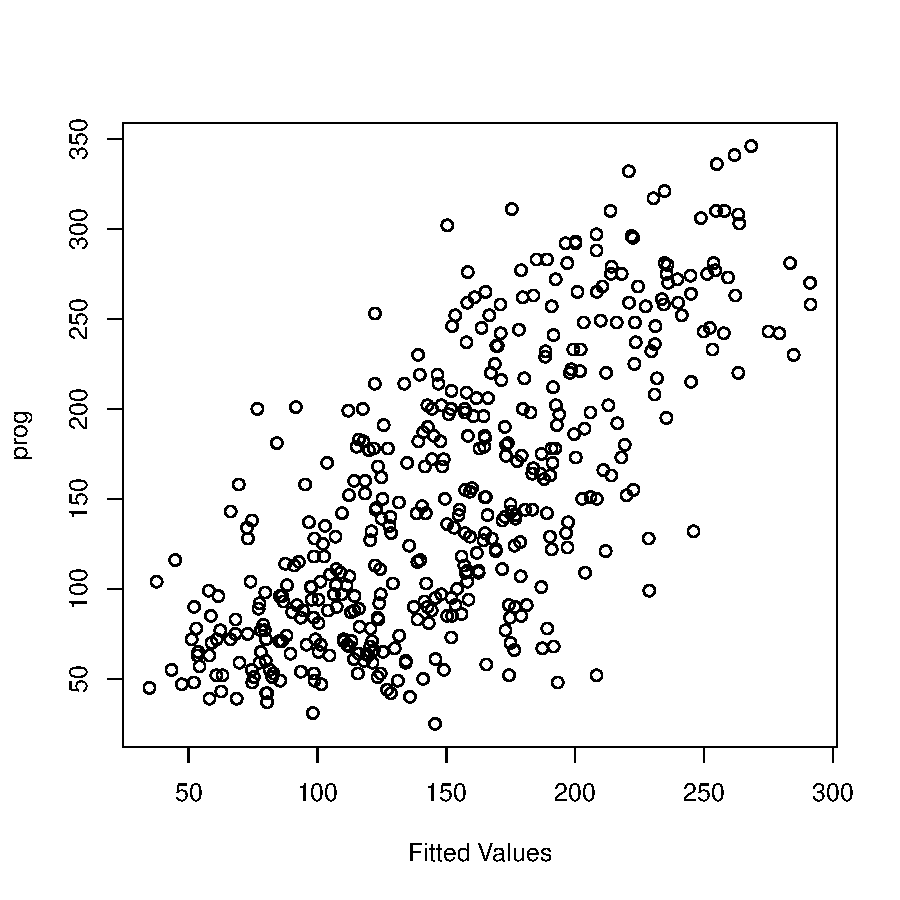
\includegraphics{RProject1_IntroToR_Diabetes-004}

\begin{Schunk}
\begin{Sinput}
> # Rescale variables to have mean 0, sd 1
> diabetes0=diabetes
> names(diabetes0)
\end{Sinput}
\begin{Soutput}
 [1] "age"  "sex"  "bmi"  "map"  "tc"   "ldl"  "hdl"  "tch"  "ltg"  "glu" 
[11] "prog"
\end{Soutput}
\begin{Sinput}
> diabetes0=apply(diabetes,2,scale)
> apply(diabetes0,2,summary)
\end{Sinput}
\begin{Soutput}
                  age           sex           bmi           map            tc
Min.    -2.251738e+00 -9.374744e-01 -1.895781e+00 -2.360223e+00 -2.662394e+00
1st Qu. -7.832846e-01 -9.374744e-01 -7.188104e-01 -7.697084e-01 -7.192046e-01
Median   1.130443e-01 -9.374744e-01 -1.529591e-01 -1.190433e-01 -9.073818e-02
Mean     6.999972e-18 -1.368253e-18  1.072178e-16 -4.778962e-16 -2.911564e-16
3rd Qu.  7.995940e-01  1.064282e+00  6.562083e-01  7.485103e-01  5.955183e-01
Max.     2.325260e+00  1.064282e+00  3.581660e+00  2.772802e+00  3.232188e+00
                  ldl           hdl           tch           ltg           glu
Min.    -2.427874e+00 -2.148448e+00 -1.604285e+00 -2.667941e+00 -2.893112e+00
1st Qu. -6.375263e-01 -7.374604e-01 -8.293610e-01 -6.859678e-01 -6.967595e-01
Median  -8.020037e-02 -1.382738e-01 -5.443750e-02 -4.733218e-02 -2.263165e-02
Mean    -1.114637e-16 -1.191685e-16 -1.414922e-16  6.008286e-16  2.365483e-16
3rd Qu.  6.267323e-01  6.155415e-01  7.204860e-01  6.793911e-01  5.862581e-01
Max.     4.174548e+00  3.804760e+00  3.889923e+00  2.793495e+00  2.847848e+00
                 prog
Min.    -1.649092e+00
1st Qu. -8.448689e-01
Median  -1.509019e-01
Mean    -1.490189e-16
3rd Qu.  7.700636e-01
Max.     2.514710e+00
\end{Soutput}
\begin{Sinput}
> apply(diabetes0,2,mean)
\end{Sinput}
\begin{Soutput}
          age           sex           bmi           map            tc 
 6.999972e-18 -1.368253e-18  1.072178e-16 -4.778962e-16 -2.911564e-16 
          ldl           hdl           tch           ltg           glu 
-1.114637e-16 -1.191685e-16 -1.414922e-16  6.008286e-16  2.365483e-16 
         prog 
-1.490189e-16 
\end{Soutput}
\begin{Sinput}
> apply(diabetes0,2,var)
\end{Sinput}
\begin{Soutput}
 age  sex  bmi  map   tc  ldl  hdl  tch  ltg  glu prog 
   1    1    1    1    1    1    1    1    1    1    1 
\end{Soutput}
\begin{Sinput}
> # Coerce matrix diabetes0 to be a data frame
> # Replace the (scaled) prog variable with 
> #     the mean-adjusted original 
> diabetes0=data.frame(diabetes0)
> diabetes0$prog=diabetes$prog - mean(diabetes$prog)
> # Check that means are 0 and variances are apply(diabetes0,2,mean)
> apply(diabetes0,2,mean)
\end{Sinput}
\begin{Soutput}
          age           sex           bmi           map            tc 
 6.999972e-18 -1.368253e-18  1.072178e-16 -4.778962e-16 -2.911564e-16 
          ldl           hdl           tch           ltg           glu 
-1.114637e-16 -1.191685e-16 -1.414922e-16  6.008286e-16  2.365483e-16 
         prog 
-1.195733e-14 
\end{Soutput}
\begin{Sinput}
> apply(diabetes0,2,var)
\end{Sinput}
\begin{Soutput}
     age      sex      bmi      map       tc      ldl      hdl      tch 
   1.000    1.000    1.000    1.000    1.000    1.000    1.000    1.000 
     ltg      glu     prog 
   1.000    1.000 5943.331 
\end{Soutput}
\begin{Sinput}
> # 3.1 Refit linear model with scaled indep vars ----
> 
> lmfit0=lm(prog~., data=diabetes0) 
> summary(lmfit0)
\end{Sinput}
\begin{Soutput}
Call:
lm(formula = prog ~ ., data = diabetes0)

Residuals:
     Min       1Q   Median       3Q      Max 
-156.308  -38.402   -0.727   38.003  151.606 

Coefficients:
              Estimate Std. Error t value Pr(>|t|)    
(Intercept) -4.004e-14  2.576e+00   0.000 1.000000    
age         -4.627e-01  2.845e+00  -0.163 0.870910    
sex         -1.139e+01  2.916e+00  -3.905 0.000109 ***
bmi          2.472e+01  3.170e+00   7.799 4.75e-14 ***
map          1.544e+01  3.116e+00   4.954 1.05e-06 ***
tc          -3.748e+01  1.983e+01  -1.890 0.059428 .  
ldl          2.248e+01  1.613e+01   1.394 0.164108    
hdl          4.758e+00  1.012e+01   0.470 0.638648    
tch          8.440e+00  7.691e+00   1.097 0.273045    
ltg          3.569e+01  8.185e+00   4.360 1.63e-05 ***
glu          3.236e+00  3.142e+00   1.030 0.303661    
---
Signif. codes:  0 '***' 0.001 '**' 0.01 '*' 0.05 '.' 0.1 ' ' 1

Residual standard error: 54.16 on 431 degrees of freedom
Multiple R-squared:  0.5176,	Adjusted R-squared:  0.5065 
F-statistic: 46.25 on 10 and 431 DF,  p-value: < 2.2e-16
\end{Soutput}
\begin{Sinput}
> 
> #   Note what statistics are same:
> #       Residual standard error
> #       Multiple R-squared 
> #       t values and p-values of indep vars
\end{Sinput}
\end{Schunk}
\begin{Schunk}
\begin{Sinput}
> # 4.  Display coefficients (estimates and confidence intervals) ----
> # Replace FALSE by TRUE if package coefplot needs to be installed
> if (FALSE){install.packages(coefplot)}
> library(coefplot)